\documentclass[12pt]{article}
\usepackage{ctex}
\usepackage{amsmath,amsthm}
\usepackage{graphicx,float}
\usepackage{fancyhdr}
\usepackage{array}
\usepackage[a4paper, total={7in,9in}]{geometry}

\graphicspath{{../image/}}

\renewcommand{\arraystretch}{1.8}

\fancyhf{}
\fancyhf[FL]{Copyright @MokOwen}
\fancyhf[FC]{\thepage}
\renewcommand{\headrulewidth}{0pt}
\renewcommand{\footrulewidth}{1pt}

\newtheorem*{theorem}{Theorem}
\newtheorem{example}{Example}
\newtheorem*{sol}{Solution}

\begin{document}
    \pagestyle{fancy}
    \begin{center}
        \textbf{Factorization}
    \end{center}

    Recall the concept of factors. From what we've learned in primary school, the factor of some number, say 18, is given by \begin{align*}
        18&=1\times 18\\
        &=2\times 9\\
        &=3\times 6
    \end{align*}
    So, in this example, we have $1,2,3,6,9,18$ as factors of $18$. Similarly, when we proceed to polynomials, the concept of factorization still works, while the computation of factorization becomes unclear and required more insights of what a polynomial is.

    Let us look at the following expressions. We know that \begin{align*}
        x\cdot x=x^2
    \end{align*} and therefore the following holds:\begin{align*}
        x^2-2x&=x(x-2)\\
        x^3+4x^2&=x^2(x+4)
    \end{align*}

    For who thinks the above expression is kind of ambiguous, let us remember the distributivity of numbers:\begin{align*}
        a(b+c)&=ab+ac\\
        (a+b)c&=ac+ab
    \end{align*} and work the expressions backward. Always equip yourself with the concept that factorization is just the reverse engineering of expansion.\begin{align*}
        x(x-2)&=x\cdot x-x\cdot 2\\
        &=x^2-2x\\
        x^2(x+4)&=x^2\cdot x+x^2\cdot 4\\
        &=x^3+4x^2
    \end{align*}

    Remember we can treat $x^2\cdot x$ as $x\cdot x\cdot x$, so 3 $x$'s multiplying together gives us $x^3$.

    However, not every polynomial is simple as we have seen. For some expressions existing in Physics, we will encounter something like:\begin{align*}
        x^2+3x+4&=0
    \end{align*}

    In order to find a way to solve for $x$, we need to learn about the methods. We will start from using identities we have learned before.

    Let's check our understanding to factorization first.
    \subsection*{Exercise}
    \begin{enumerate}
        \item List out all factors for the following numbers, including negatives:\begin{align*}
            &a)\ 4&&b)\ 6&&c)\ 12&&d)\ 15\\
            &e)\ 32&&f)\ 44&&g)\ 52&&h)\ 80
        \end{align*}
        \item Factorize the following by prime factorization:\begin{align*}
            &a)\ 4&&b)\ 6&&c)\ 12&&d)\ 15\\
            &e)\ 32&&f)\ 44&&g)\ 52&&h)\ 80
        \end{align*}
        \item Factorize the following:\begin{align*}
            &a)\ x^2+x&&b)\ x-xy&&c)\ x^4+2x^2+2x&&d)\ x^3-2x
        \end{align*}
    \end{enumerate}

    \begin{center}
        \textbf{Factorization using identities}
    \end{center}

    Recall the following expansion:\begin{align*}
        (x+y)^2&=x^2+2xy+y^2\\
        (x-y)^2&=x^2-2xy+y^2\\
        (x+y)(x-y)&=x^2-y^2
    \end{align*}

    We should always notice that the equal sign = is two-way meaningful, that is, whenever the left-hand side is equal to the right-hand side, the right-hand side is immediately equal to the left-hand side. Therefore, we may see the above in a reverse direction.\begin{align*}
        x^2+2xy+y^2&=(x+y)^2\\
        x^2-2xy+y^2&=(x-y)^2\\
        x^2-y^2&=(x+y)(x-y)
    \end{align*}

    This is called the \textbf{factorization with identities}.

    \begin{example}
        Factorize $x^2+2x+1$.
    \end{example}
    \textit{ Sol. }\begin{align*}
        x^2+2x+1&=(x)^2+2(x)(1)+(1)^2\\
        &=(x+1)^2
    \end{align*}

    \begin{example}
        Factorize $x^2+4x+4$.
    \end{example}
    \textit{ Sol. }\begin{align*}
        x^2+4x+4&=(x)^2+2(x)(2)+(2)^2\\
        &=(x+2)^2
    \end{align*}

    \begin{example}
        Factorize $x^2-2x+1$.
    \end{example}
    \textit{ Sol. }\begin{align*}
        x^2-2x+1&=(x)^2-2(x)(1)+(1)^2\\
        &=(x-1)^2
    \end{align*}

    \begin{example}
        Factorize $x^2-4x+4$.
    \end{example}
    \textit{ Sol. }\begin{align*}
        x^2-4x+4&=(x)^2-2(x)(2)+(2)^2\\
        &=(x-2)^2
    \end{align*}

    \begin{example}
        Factorize $x^2-1$.
    \end{example}
    \textit{ Sol. }\begin{align*}
        x^2-1&=(x)^2-(1)^2\\
        &=(x+1)(x-1)
    \end{align*}

    \begin{example}
        Factorize $x^2-9$.
    \end{example}
    \textit{ Sol. }\begin{align*}
        x^2-9&=(x)^2-(3)^2\\
        &=(x+3)(x-3)
    \end{align*}

    We shall now be familiar with simple factorization. Let's practise with these basic identities.

    \subsection*{Exercise}
    \begin{enumerate}
        \item Factorize the following:\begin{align*}
            &a)\ x^2+6x+9&&b)\ x^2+8x+16&&c)\ x^2+10x+25&&d)\ x^2+16x+64\\
            &e)\ 2x^2+12x+18&&f)\ 4x^2+32x+64&&g)\ 6x^2+60x+150&&h)\ 8x^2+128x+512\\
            &i)\ x^3+6x^2+9x&&j)\ x^5+8x^4+16x^3&&k)\ x^8+10x^6+25x^4&&l)\ x^9+16x^5+64x\\
        \end{align*}
        \item Factorize the following:\begin{align*}
            &a)\ x^2-6x+9&&b)\ x^2-8x+16&&c)\ x^2-10x+25&&d)\ x^2-16x+64\\
            &e)\ 2x^2-12x+18&&f)\ 4x^2-32x+64&&g)\ 6x^2-60x+150&&h)\ 8x^2-128x+512\\
            &i)\ x^3-6x^2+9x&&j)\ x^5-8x^4+16x^3&&k)\ x^8-10x^6+25x^4&&l)\ x^9-16x^5+64x\\
        \end{align*}
        \item Factorize the following:\begin{align*}
            &a)\ x^2-9&&b)\ x^2-16&&c)\ x^2-25&&d)\ x^2-64\\
            &e)\ 2x^2-18&&f)\ 4x^2-64&&g)\ 6x^2-150&&h)\ 8x^2-512\\
            &i)\ x^3-9x&&j)\ x^5-16x^3&&k)\ x^8-25x^4&&l)\ x^9-64x\\
        \end{align*}
        \item Factorize the following:\begin{align*}
            &a)\ x^2+2ax+a^2&&b)\ x^2+8x+16-b^2\\
            &c)\ x^2+10x+25+y^2-2c+c^2&&d)\ ax^2+16a^2x+64a^3\\
            &e)\ 2x^2+12xy+18y^2&&f)\ 4(x+y)^2+32(x^2-y^2)+64(x-y)^2
        \end{align*}
    \end{enumerate}

    \begin{center}
        \textbf{Factorization using more identities}
    \end{center}

    For more information to using identities, we will learn more expressions to familiarize ourselves with them.

    We had expressions of degree 2, so we could also proceed to that of degree 3.\begin{align*}
        (x+y)^3&=x^3+3x^2y+3xy^2+y^3\\
        (x-y)^3&=x^3-3x^2y+3xy^2-y^3\\
        (x+y)(x^2-xy+y^2)&=x^3+y^3\\
        (x-y)(x^2+xy+y^2)&=x^3-y^3
    \end{align*}

    Just, to be clear of what is happening, we will give the expansions a clear proof.\begin{enumerate}
        \item For $(x+y)^3=x^3+3x^2y+3xy^2+y^3$:\begin{align*}
            (x+y)^3&=(x+y)(x+y)^2\\
            &=(x+y)(x^2+2xy+y^2)\\
            &=x^3+3x^2y+3xy^2+y^3
        \end{align*}
        \item For $(x-y)^3=x^3-3x^2y+3xy^2-y^3$:\begin{align*}
            (x-y)^3&=(x-y)(x-y)^2\\
            &=(x-y)(x^2-2xy+y^2)\\
            &=x^3-3x^2y+3xy^2-y^3
        \end{align*}
        \item For $(x+y)(x^2-xy+y^2)=x^3+y^3$:\begin{align*}
            (x+y)(x^2-xy+y^2)&=x^3+x^2y-x^2y-xy^2+xy^2+y^3\\
            &=x^3+y^3
        \end{align*}
        \item For $(x-y)(x^2+xy+y^2)=x^3-y^3$:\begin{align*}
            (x-y)(x^2+xy+y^2)&=x^3-x^2y+x^2y-xy^2+xy^2-y^3\\
            &=x^3-y^3
        \end{align*}
    \end{enumerate}
    
    Let's look at some examples to familiarize ourselves to how these work.

    \begin{example}
        Factorize $x^3+3x^2+3x+1$.
    \end{example}
    \textit{ Sol. }\begin{align*}
        x^3+3x^2+3x+1&=(x)^3+3(x)^2(1)+3(x)(1)^2+(1)^3\\
        &=(x+1)^3
    \end{align*}

    \begin{example}
        Factorize $x^3+6x^2+12x+8$.
    \end{example}
    \textit{ Sol. }\begin{align*}
        x^3+6x^2+12x+8&=(x)^3+3(x)^2(2)+3(x)(2)^2+(2)^3\\
        &=(x+2)^3
    \end{align*}

    \begin{example}
        Factorize $x^3-3x^2+3x-1$.
    \end{example}
    \textit{ Sol. }\begin{align*}
        x^3-3x^2+3x-1&=(x)^3-3(x)^2(1)+3(x)(1)^2-(1)^3\\
        &=(x-1)^3
    \end{align*}

    \begin{example}
        Factorize $x^3-6x^2+12x-8$.
    \end{example}
    \textit{ Sol. }\begin{align*}
        x^3-6x^2+12x-8&=(x)^3-3(x)^2(2)+3(x)(2)^2-(2)^3\\
        &=(x-2)^3
    \end{align*}

    \begin{example}
        Factorize $x^3+1$.
    \end{example}
    \textit{ Sol. }\begin{align*}
        x^3+1&=(x)^3+(1)^3\\
        &=(x+1)(x^2-x+1)
    \end{align*}

    \begin{example}
        Factorize $x^3+8$.
    \end{example}
    \textit{ Sol. }\begin{align*}
        x^3+8&=(x)^3+(2)^3\\
        &=(x+2)(x^2-2x+4)
    \end{align*}

    \begin{example}
        Factorize $x^3-1$.
    \end{example}
    \textit{ Sol. }\begin{align*}
        x^3-1&=(x)^3-(1)^3\\
        &=(x-1)(x^2+x+1)
    \end{align*}

    \begin{example}
        Factorize $x^3-8$.
    \end{example}
    \textit{ Sol. }\begin{align*}
        x^3-8&=(x)^3-(2)^3\\
        &=(x-2)(x^2+2x+4)
    \end{align*}

    We shall now be familiar with degree 3 factorization. Let's practise with these basic identities.

    \subsection*{Exercise}
    \begin{enumerate}
        \item Factorize the following:\begin{align*}
            &a)\ x^3+9x^2+27x+81&&b)\ x^3+12x^2+48x+64&&c)\ x^3+15x^2+75x+125\\
            &d)\ 2x^3+18x^2+54x+162&&e)\ 3x^3+36x^2+144x+192&&f)\ 5x^3+75x^2+375x+625\\
        \end{align*}
        \item Factorize the following:\begin{align*}
            &a)\ x^3-9x^2+27x-81&&b)\ x^3-12x^2+48x-64&&c)\ x^3-15x^2+75x-125\\
            &d)\ 2x^3-18x^2+54x-162&&e)\ 3x^3-36x^2+144x-192&&f)\ 5x^3-75x^2+375x-625\\
        \end{align*}
        \item Factorize the following:\begin{align*}
            &a)\ x^3+81&&b)\ x^3+12x^2+48x+64&&c)\ x^3+125\\
            &d)\ 2x^3+162&&e)\ 3x^3+192&&f)\ 5x^3+625\\
        \end{align*}
        \item Factorize the following:\begin{align*}
            &a)\ x^3-81&&b)\ x^3-64&&c)\ x^3-125\\
            &d)\ 2x^3-162&&e)\ 3x^3-192&&f)\ 5x^3-625\\
        \end{align*}
    \end{enumerate}

    \begin{center}
        \textbf{Factorization using cross-method}
    \end{center}

    From now on, we will dive into the main question: How to factorize any quadratic (degree 2) polynomials in the form of $$x^2+px+q$$ or, to be more general, $$ax^2+bx+c$$ using rational thinking? We shall now suppose if a quadratic polynomial $x^2+px+q$ can be factorized into the form $$(x+a)(x+b)$$ then it is equivalent to saying $$(x+a)(x+b)=x^2+px+q$$ which if we proceed one step further, the result will be $$x+(a+b)x+ab=x^2+px+q$$

    It should be clear to see that \begin{align*}
        \begin{cases}
            a+b=p\\
            ab=q
        \end{cases}
    \end{align*}

    This then gives us a hint that we should perform a factorization on the constant $q$ first, then try to figure out which pair of $a,b$ gives the true relation on $a+b=p$.

    So we may now conclude the steps of investigation and familiarize ourselves with some examples.\begin{enumerate}
        \item By comparing like terms, discover the $p,q$ in the expressions.
        \item Try to factorize $q$, state every pair of factors.
        \item Check the sum of each pair of factors. If one provides a true result on $a+b=p$, then it is the true pair we need.
        \item Write down $(x+a)(x+b)$ as the factorized form.
    \end{enumerate}

    \begin{example}
        Factorize $x^2+4x+3$.
    \end{example}

    \textit{ Sol.}Step 1: find $p$ and $q$.
    \begin{align*}
        p=4, q=3
    \end{align*}
    \indent \indent Step 2: Factorize $q$ (with negative pairs).
    \begin{align*}
        3&=1\cdot 3\\
        &=(-1)\cdot(-3)
    \end{align*}
    \indent \indent Step 3: Check $a+b=p$ (with negative pairs).
    \begin{align*}
        1+3&=4\\
        (-1)+(-3)&=-4
    \end{align*}
    \indent \indent \indent Since $p=4$, we have the factor pair $a=1,b=3$.\\
    \indent \indent Step 4: Complete the factorization.
    \begin{align*}
        x^2+4x+3=(x+1)(x+3)
    \end{align*}

    We could check that the factorized expression is indeed expanding back to the original polynomial.\begin{align*}
        (x+1)(x+3)&=x(x+3)+(x+3)\\
        &=x^2+3x+x+3\\
        &=x^2+4x+3
    \end{align*}

    This shows that our work is correctly given. Someone in the history consider the above steps could be refined in a compressed way of representation. We shall call it the \textbf{cross-method}.
    
    \begin{example}
        Factorize $x^2+4x+3$ using cross-method.
    \end{example}

    \textit{ Sol.}As long as $3=1\cdot 3=(-1)\cdot(-3)$, we have 
    \begin{figure}[H]
        \centering
        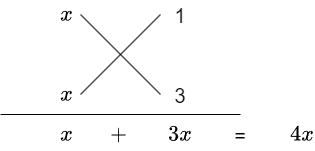
\includegraphics[scale=0.6]{cross-method}
    \end{figure}
    \indent \indent That is, the factorization shows $x^2+4x+3=(x+1)(x+3)$.

    From here, you should be familiar enough to cross-method. You may check your understanding of using cross-method by the following exercises.

    \subsection*{Exercise}
    \begin{enumerate}
        \item Factorize the following using cross-method:\begin{align*}
            &a)\ x^2+6x+8&&b)\ x^2+9x+18&&c)\ x^2+7x+6\\
            &d)\ x^2-6x+8&&e)\ x^2-9x+18&&f)\ x^2-7x+6\\
            &g)\ x^2+6x-27&&h)\ x^2+9x-22&&i)\ x^2+7x-30\\
            &j)\ x^2-6x-27&&k)\ x^2-9x-22&&l)\ x^2-7x-30
        \end{align*}
        \item Factorize the following using cross-method:\begin{align*}
            &a)\ 2x^2+12x+16&&b)\ 3x^2+27x+54&&c)\ 5x^2+35x+30\\
            &d)\ 7x^2-42x+56&&e)\ -11x^2+99x-198&&f)\ -3x^2+21x-18
        \end{align*}
    \end{enumerate}

    \begin{center}
        \textbf{Solving quadratic equations by factor method}
    \end{center}

    To solve quadratic equations, we acknowledge the following:\begin{theorem}
        If $ab=0$, then either $a=0$ or $b=0$.
    \end{theorem}

    It should be clear that from above theorem, we have when $(x-\alpha)(x-\beta)=0$, then $x-\alpha=0$ or $x-\beta=0$. This means the \textbf{solutions} to the equation are $x=\alpha$ or $x=\beta$.

    \begin{example}
        Solve $x^2-4x+3=0$.
    \end{example}

    \textit{ Sol. }By factorization, we have $(x-1)(x-3)=0$, then $x=1$ or $x=3$ are the solutions to the equation.

    \begin{example}
        Solve $x^2+4x+3=0$.
    \end{example}

    \textit{ Sol. }By factorization, we have $(x+1)(x+3)=0$, then $x=-1$ or $x=-3$ are the solutions to the equation.

    We may also encounter double roots, i.e. duplicated solution to the equation. Then we can write the solution once only.

    \begin{example}
        Solve $x^2+4x+4=0$.
    \end{example}

    \textit{ Sol. }By factorization, we have $(x+2)^2=0$, then $x=-2$ is the solution to the equation.

    \subsection*{Exercise}
    \begin{enumerate}
        \item Solve the following equations:\begin{align*}
            &a)\ 2x^2+12x+16=0&&b)\ 3x^2+27x+54=0&&c)\ 5x^2+35x+30=0\\
            &d)\ 7x^2-42x+56=0&&e)\ -11x^2+99x-198=0&&f)\ -3x^2+21x-18=0
        \end{align*}
        \item Solve the following equations:\begin{align*}
            &a)\ x^2+6x+9=0&&b)\ x^2+8x+16=0&&c)\ x^2+10x+25=0\\
            &d)\ x^2+16x+64=0&&e)\ 2x^2-12x+18=0&&f)\ 4x^2-32x+64=0\\
            &g)\ 6x^2-60x+150=0&&h)\ 8x^2-128x+512=0&&i)\ x^3-9x=0\\
            &j)\ x^5-16x^3=0&&k)\ x^8-25x^4=0&&l)\ x^9-64x=0
        \end{align*}
    \end{enumerate}

    \begin{center}
        \textbf{Solving quadratic equations using formula}
    \end{center}

    One should observe that not every quadratic polynomial can be factorized perfectly. For example, if the equation be like:$$x^2+6x-6=0$$

    We could see for the left-hand side, if $x=0$, the expression computes $<0$; if $x=1$, the expression computes $>0$. You could imagine there must be some number $0<x<1$ so that the equation holds.
    
    For exact solution, one introduced the notation $\sqrt{k}$ for finding the solution to $x^2=k$. It is important to remember that both positive and negative numbers can be squared to become positive, i.e. $(\sqrt{x})^2=x$ and $(-\sqrt{x})^2=x$ if $x>0$.

    For any quadratic equation in the form of $ax^2+bx+c=0$, one provides a solution in the following form:$$\frac{-b\pm\sqrt{b^2-4ac}}{2a}$$where the plus or minus sign $\pm$ indicates two solutions in one writing. This means the above formula is representing, if $x$ satisfies the equation, then either $$x=\frac{-b+\sqrt{b^2-4ac}}{2a}\textrm{ or }x=\frac{-b-\sqrt{b^2-4ac}}{2a}$$ 
    
    The origination of the formula comes from completing square method, which is quite hard to understand. We will write it down abstractly as for the proof of quadratic formula, and concrete examples will be introduced later in the section of graphs of quadratic polynomials.

    Here's the proof of quadratic formula:\begin{align*}
        ax^2+bx+c&=0\\
        a(x^2+\frac{b}{a}x)+c&=0\\
        a(x^2+2\frac{b}{2a}x+\frac{b^2}{4a^2}-\frac{b^2}{4a^2})+c&=0\\
        a(x+\frac{b}{2a})^2&=\frac{b^2-4ac}{4a}\\
        (x+\frac{b}{2a})^2&=\frac{b^2-4ac}{4a^2}\\
        x+\frac{b}{2a}&=\pm\frac{\sqrt{b^2-4ac}}{2a}\\
        x&=\frac{-b\pm\sqrt{b^2-4ac}}{2a}
    \end{align*}

    We will go through some usage of quadratic formula.

    \begin{example}
        Solve $x^2+7x-9=0$ using quadratic formula.
    \end{example}

    \textit{ Sol.} Identifying $a=1$, $b=7$, $c=-9$, we have \begin{align*}
        x&=\frac{-b\pm\sqrt{b^2-4ac}}{2a}\\
        &=\frac{-7\pm\sqrt{7^2-4\cdot 1\cdot (-9)}}{2}\\
        &=\frac{-7\pm\sqrt{85}}{2}
    \end{align*}

    \begin{example}
        Solve $2x^2+3x-4=0$ using quadratic formula.
    \end{example}

    \textit{ Sol.} Identifying $a=2$, $b=3$, $c=-4$, we have \begin{align*}
        x&=\frac{-b\pm\sqrt{b^2-4ac}}{2a}\\
        &=\frac{-3\pm\sqrt{3^2-4\cdot 2\cdot (-4)}}{4}\\
        &=\frac{-3\pm\sqrt{41}}{4}
    \end{align*}

    You may now try to solve any quadratic equation using quadratic formula.

    \subsection*{Exercise}

    \begin{enumerate}
        \item Solve the following quadratic equation:\begin{align*}
            &a)\ 3x^2-12x-26=0&&b)\ 7x^2-27x+54=0&&c)\ 4x^2+35x+1=0\\
            &d)\ 2x^2-33x+6=0&&e)\ -11x^2+89x-18=0&&f)\ -3x^2+21x-18=0
        \end{align*}
        \item Solve the following quadratic equation in terms of $k$:\begin{align*}
            &a)\ 3kx^2-x-2=0&&b)\ 7x^2-27x+k=0&&c)\ kx^2+35x+1=0\\
            &d)\ 2x^2-3kx+6=0&&e)\ -11x^2+kx-k=0&&f)\ -kx^2+21x-k^2=0
        \end{align*}
    \end{enumerate}

    \begin{center}
        \textbf{Nature of roots: the existence of real roots}
    \end{center}

    One should observe that the quadratic formula $$\frac{-b\pm \sqrt{b^2-4ac}}{2a}$$ consists of a square-root part, namely $b^2-4ac$, that affects the nature of roots very much. We gave it a name as \textbf{discriminant}, meaning the value of it discriminates the nature of roots. If this part is $\geq 0$, the quadratic formula returns a real number; if this part is $< 0$, then we will be facing a square-root of negative numbers. From the history it kills a lot of mathematicians, but from now on let us define a new notion for it.

    We will define a new element call $i$ such that it satisfies the equation $$i^2=-1$$ and such that for any positive real number $k$, we can write $\sqrt{-k}=i\sqrt{k}$. We shall call $i$ the imaginary number as it could not be thought of as a real number. For something unreal, that is imaginary.

    In this sense, for if $b^2-4ac<0$, we could have a suitable form of writing, in the form of $x+yi$, so that every solution to quadratic equation is well-written. We call this form of number a \textbf{complex number}, with $x,y$ to be some real numbers.

    From here let us write down the conclusion to the reality of roots using a table:

    \begin{center}
        \begin{tabular}{|c|c|c|}
            \hline
            $\Delta=b^2-4ac$&Roots&Nature of roots\\
            \hline
            $>0$&$\dfrac{-b\pm\sqrt{\Delta}}{2a}$&2 distinct real roots\\
            \hline
            $=0$&$\dfrac{-b}{2a}$&1 double root\\
            \hline
            $<0$&$\dfrac{-b\pm\sqrt{-\Delta}i}{2a}$&No real roots (2 complex roots)\\
            \hline
        \end{tabular}
    \end{center}

    From this we can now easily determine the nature of roots before really computing the value of the roots.

    \begin{example}
        Determine the nature of roots of the following. If it has real root(s), solve for it.\begin{enumerate}
            \item[(a)] $7x^2+5x-10=0$.
            \item[(b)] $81x^2-18x+1=0$.
            \item[(c)] $20x^2+19x+10=0$.
        \end{enumerate}
    \end{example}

    \textit{ Sol.}\begin{enumerate}
        \item[(a)] Checking the discriminant $\Delta=b^2-4ac=5^2-4(7)(-10)=305>0$, so it has 2 distinct real roots. By substituting the $\Delta$ back to the quadratic formula, we have \begin{align*}
            x=\frac{-b\pm\sqrt{\Delta}}{2a}=\frac{-5\pm\sqrt{305}}{14}
        \end{align*}
        \item[(b)] Checking the discriminant $\Delta=b^2-4ac=(-18)^2-4(81)(1)=0$, so it has 1 double real root. By substituting the $\Delta$ back to the quadratic formula, we have \begin{align*}
            x=\frac{-b}{2a}=\frac{18}{162}=\frac{1}{9}
        \end{align*}
        \item[(c)] Checking the discriminant $\Delta=b^2-4ac=19^2-4(20)(10)=-439<0$, so it has no real roots. 
    \end{enumerate}

    We also notice that if we know the nature of roots for some unknown quadratic equations, we could retrieve the unknowns by drawing out propositions on the discriminant.

    \begin{example}
        It is known that the quadratic equation $kx^2-4x+k=0$ has only one real root, with real number $k$. Solve the equation.
    \end{example}

    \textit{ Sol.}By checking the discriminant, we obtain the following:\begin{align*}
        (-4)^2-4\cdot k\cdot k&=0\\
        k&=\pm 2
    \end{align*}
    \indent \indent Therefore, the equation should be either $2x^2-4x+2=0$ or $-2x^2-4x-2=0$, and correspondingly having $x=2$ and $x=-2$ as root respectively.

    \subsection*{Exercise}
    \begin{enumerate}
        \item Determine the nature of roots of the following quadratic equation:\begin{align*}
            &a)\ -390x^2-988x+794=0&&b)\ 82x^2+290x+759=0&&c)\ -924x^2-708x+959=0\\
            &d)\ -265x^2+336x-685=0&&e)\ 845x^2+396x-501=0&&f)\ -246x^2+16x-318=0
        \end{align*}
        \item If the following quadratic equations all have only one real root, find the value(s) of $k$.\begin{align*}
            &a)\ kx^2-2x+9=0&&b)\ 82x^2+kx+79=0&&c)\ -24x^2-70x+4k=0\\
            &d)\ -kx^2+36x-k=0&&e)\ 8kx^2+3kx-51=0&&f)\ 2kx^2+(3k-6)x-4k-8=0
        \end{align*}
    \end{enumerate}

    \begin{center}
        \textbf{Vieta's formula: relation between roots and coefficients}
    \end{center}

    We can now further dive into some kind of abstract-nonsense. In previous section, we found that discriminant tells us the nature of the roots of the quadratic equation, and if we see the roots counted with multiplicity, the number of roots is always being equal to 2. This is not so surprising because we can always think of factorizing a quadratic equation into a product of two linear factors, so our work could be done by assuming there is always 2 roots, either they are the same or distinct.

    We shall now investigate the relation between roots and coefficients, so we have a new game created by Mathematicians called algebra. Let us assume that we have a quadratic equation in the form of $x^2+px+q=0$, and this equation has roots $\alpha$ and $\beta$, which may not be real but we could still represent them using complex numbers. For if we translate the words into mathematical presentation: $$(x-\alpha)(x-\beta)=0=x^2-px+q$$ It is clear that the left-hand side is exactly equal to the right-hand side. We then expand the left-hand side to the following form: $$x^2-(\alpha+\beta)x+\alpha\beta=x^2+px+q$$ This takes us to the relation between roots and coefficients by comparing like terms $$\begin{cases}
        \alpha+\beta=-p\\ 
        \alpha\beta=q
    \end{cases}$$

    The simultaneous equations above is a system of relation called the \textbf{Vieta's formula}, which has another name called the \textbf{sum of roots} for the first equation and \textbf{product of roots} for the second equation.

    In order to generalize the relationship further to any quadratic equations in the form of $ax^2+bx+c=0$ with real numbers $a,b,c$, we take the following transformation $$ax^2+bx+c=0 \implies x^2+\frac{b}{a}x+\frac{c}{a}=0$$ so that the equation is identical to what we have investigated just a moment before by taking $p=\frac{b}{a}$ and $q=\frac{c}{a}$. Therefore, the general Vieta's formula becomes $$\begin{cases}
        \alpha+\beta=-\frac{b}{a}\\ 
        \alpha\beta=\frac{c}{a}
    \end{cases}$$

    \begin{example}
        Find the sum of roots and product of roots for the quadratic equation $3x^2+2x+9=0$.
    \end{example}

    \textit{ Sol.}By letting $\alpha$ and $\beta$ to be the roots of the equation, using Vieta's formula we get $$\begin{cases}
        \alpha+\beta=-\frac{2}{3}\\ 
        \alpha\beta=\frac{9}{3}=3
    \end{cases}$$

    \begin{example}
        Construct a quadratic equation with integral coefficients using $\frac{1}{2}$ and $\frac{2}{3}$ as roots.
    \end{example}

    \textit{ Sol.}Using Vieta's formula we get $$\begin{cases}
        \alpha+\beta=\frac{1}{2}+\frac{2}{3}=\frac{5}{6}\\ 
        \alpha\beta=\frac{1}{2}\cdot \frac{2}{3}=\frac{1}{3}
    \end{cases}$$
    \indent \indent Hence, the quadratic equation we need is given by $$x^2-(\alpha+\beta)x+\alpha\beta=0 \implies x^2-\frac{5}{6}x+\frac{1}{3}=0 \implies 6x^2-5x+2=0$$

    \subsection*{Exercise}
    \begin{enumerate}
        \item Find the sum of roots and product of roots for the following quadratic equations:\begin{align*}
            &a)\ -390x^2-988x+794=0&&b)\ 82x^2+290x+759=0&&c)\ -924x^2-708x+959=0\\
            &d)\ -265x^2+336x-685=0&&e)\ 845x^2+396x-501=0&&f)\ -246x^2+16x-318=0\\
            &g)\ kx^2-2x+9=0&&h)\ 82x^2+kx+79=0&&i)\ -24x^2-70x+4k=0\\
            &j)\ -kx^2+36x-k=0&&k)\ 8kx^2+3kx-51=0&&l)\ 2kx^2+(3k-6)x-4k-8=0
        \end{align*}
        \item Construct, for each pair of roots stated below, a quadratic equation with integral coefficients respectively.\begin{enumerate}
            \item $\frac{2}{5}$ and $-\frac{6}{7}$.
            \item $\frac{3}{2}$ and $\frac{7}{4}$.
            \item $4$ and $-4$.
            \item $5$ and $-\frac{2}{7}$.
        \end{enumerate}
    \end{enumerate}

    \begin{center}
        \textbf{More about roots of equations (Optional)}
    \end{center}

    To construct a quadratic equation, we shall first figure out the roots of the required polynomial. Most of the times we are not going to be given roots, but we will need to compute from other given information.

    \begin{example}
        It is given that $\alpha$ and $\beta$ are roots of the quadratic polynomial $ax^2+bx+c$. Construct a quadratic polynomial with roots $\alpha^2$ and $\beta^2$ in terms of $a,b,c$.
    \end{example}

    \textit{ Sol.} To construct the required polynomial we shall find by Vieta's formula the value of $\alpha^2+\beta^2$ and $\alpha^2\beta^2$. It is known that from our assumption that \begin{align*}
        \begin{cases}
            \alpha+\beta=-\frac{b}{a}\\
            \alpha\beta=\frac{c}{a}
        \end{cases}
    \end{align*}
    Therefore, the required sum of roots and product of roots are \begin{align*}
        \alpha^2+\beta^2&=(\alpha+\beta)^2-2\alpha\beta=\frac{b^2-2ac}{a^2}\\
        \alpha^2\beta^2&=(\alpha\beta)^2=\frac{c^2}{a^2}
    \end{align*}
    which means the required polynomial is $$a^2x^2+(2ac-b^2)x+c^2$$

    \begin{example}
        It is given that $\begin{cases}
                \beta^2-3\beta+2=0\\
                \alpha^2-3\alpha+2=0
            \end{cases}$, find the value of $(\alpha+1)(\beta+1)$.
    \end{example}

    \textit{ Sol.} The given condition is equivalent to saying $\alpha$ and $\beta$ are roots to the equation $x^2-3x+2$, hence by Vieta's formula we have \begin{align*}
        \begin{cases}
            \alpha+\beta=3\\
            \alpha\beta=2
        \end{cases}
    \end{align*}
    Then we may compute the answer:\begin{align*}
        (\alpha+1)(\beta+1)&=\alpha\beta+(\alpha+\beta)+1\\
        &=2+3+1\\
        &=6
    \end{align*}

    \begin{example}
        It is given that $\alpha$ and $\beta$ are real roots of the quadratic polynomial $ax^2+bx+c$, where $\alpha<\beta$. Find the following in terms of $a,b,c$.\begin{align*}
            &a)\ \beta-\alpha&&b)\ \alpha^2-\beta^2&&c)\ \alpha^3+\beta^3\\
            &d)\ a\beta^2+b\beta&&e)\ a\beta^2-b\alpha&&f)\ a(\beta-\alpha)^2+b(\beta+\alpha)+c
        \end{align*}
    \end{example}

    \textit{ Sol.}\begin{enumerate}
        \item[(a)] \begin{align*}
            (\beta-\alpha)^2&=(\alpha+\beta)^2-4\alpha\beta\\
            &=\frac{b^2-4ac}{a^2}\\
            \beta-\alpha&=\frac{\sqrt{b^2-4ac}}{|a|}&(\beta-\alpha>0)
        \end{align*} 
        \item[(b)] \begin{align*}
            \alpha^2-\beta^2&=(\alpha-\beta)(\alpha+\beta)\\
            &=-\frac{\sqrt{b^2-4ac}}{|a|}\cdot \frac{-b}{a}\\
            &=\frac{b\sqrt{b^2-4ac}}{a|a|}
        \end{align*}
        \item[(c)] \begin{align*}
            \alpha^3+\beta^3&=(\alpha+\beta)(\alpha^2-\alpha\beta+\beta^2)\\
            &=(\alpha+\beta)((\alpha+\beta)^2-3\alpha\beta)\\
            &=(-\frac{b}{a})((-\frac{b}{a})^2-3\frac{c}{a})\\
            &=\frac{3abc-b^3}{a^3}
        \end{align*}
        \item[(d)] $a\beta^2+b\beta=a\beta^2+b\beta+c-c=-c$.
        \item[(e)] $\displaystyle a\beta^2-b\alpha=(a\beta^2+b\beta+c)-b\alpha-b\beta-c=-b(\alpha+\beta)-c=\frac{b^2}{a}-c=\frac{b^2-ac}{a}$.
        \item[(f)] \begin{align*}
            a(\beta-\alpha)^2+b(\beta+\alpha)+c&=a\beta^2-2a\alpha\beta+a\alpha^2+b\beta+b\alpha+c\\
            &=(a\beta^2+b\beta+c)+(a\alpha^2+b\alpha+c)-2a\alpha\beta-c\\
            &=2b-c
        \end{align*}
    \end{enumerate}

    \begin{center}
        \textbf{Graph of quadratic equations}
    \end{center}

    Let us now understand what is in fact a quadratic polynomial. Usually, we say a quadratic curve is a parabola, which comes up in Physics studies about motion of throwing an object.

    \begin{figure}[H]
        \centering
        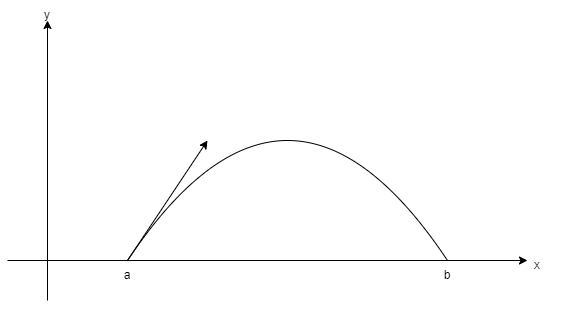
\includegraphics[scale=0.8]{parabola.png}
    \end{figure}

    Seeing the y-axis as the tag for height from the ground, and seeing x-axis as the tag for horizontal distance, we obtain a trajectory for a throwing motion starting from $x=a$ to $x=b$ in the direction indicated by an arrow drawn on the figure. Recall some memory of speed and distance, we have \begin{align*}
        x-a=v_x t
    \end{align*}where $v_x$ indicates the horizontal speed. This modelling satisfies the condition for when $t=0$, $x=a$, and that $v_x$ is constant. We now have $t$ to be the tag for time and we know that the whole motion shares the same time tag, which means for vertical component (i.e. the height) also undergoes the same time parameter $t$, so that \begin{align*}
        v_y=u_y-gt
    \end{align*}
    is a suitable modelling for the vertical component in which is meaning the vertical velocity is decreasing consistently with respect to the gravity. By the understanding from physicists that \begin{align*}
        y=\frac{u_y+v_y}{2}t
    \end{align*} we have the equation \begin{align*}
        y=u_y t-\frac{1}{2}gt^2
    \end{align*} and by simple substitution of $t=\frac{x-a}{v_x}$ into the equation for $y$ we have an equation for parabola in the form of \begin{align*}
        y=ax^2+bx+c
    \end{align*}

    To investigate the properties of a quadratic curve we introduce the \textbf{method of completing square}:\begin{align*}
        ax^2+bx+c&=a(x^2+\frac{b}{a}x)+c\\
        &=a(x^2+2\frac{b}{2a}x+\frac{b^2}{4a^2}-\frac{b^2}{4a^2})+c\\
        &=a(x+\frac{b}{2a})^2-\frac{b^2-4ac}{4a}\\
        &=a(x+\frac{b}{2a})^2+\frac{4ac-b^2}{4a}
    \end{align*}

    One observation is that when $x+\dfrac{b}{2a}$ attains 0, the polynomial attains its extremum value (maximum or minimum), because for $(x+\frac{b}{2a})^2$ its minimum value is 0, and the polynomial in this form can be controlled by $x+\frac{b}{2a}$. The above form is called the \textbf{vertex form}. Using the vertex form, we can now conclude: \begin{itemize}
        \item The \textbf{vertex} is at $(-\dfrac{b}{2a},\dfrac{4ac-b^2}{4a})$.
        \item The \textbf{axis of symmetry} is $x=-\dfrac{b}{2a}$.
        \item The \textbf{extremum value} is $\dfrac{4ac-b^2}{4a}$.
    \end{itemize}

    We may also notice that when the graph has minimum point, it should be opening upward:

    \begin{figure}[H]
        \centering
        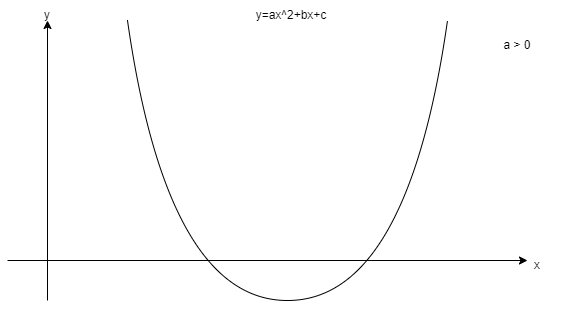
\includegraphics[scale=0.6]{open_upward.png}
    \end{figure}

    and when the graph has maximum point, it should be opening downward:

    \begin{figure}[H]
        \centering
        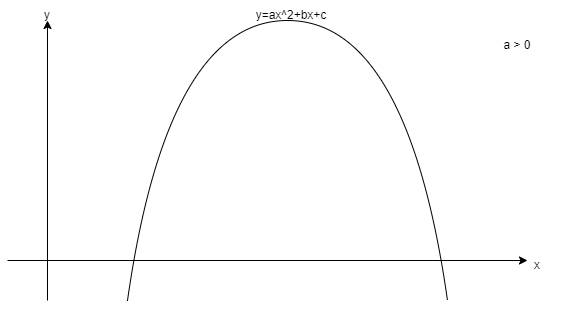
\includegraphics[scale=0.6]{open_downward.png}
    \end{figure}

    \begin{example}
        Using the method of completing square, determine the direction of opening, and find the vertex, axis of symmetry and the minimum value for the graph of $y=2x^2+3x+4$.
    \end{example}

    \textit{ Sol.}\begin{align*}
        2x^2+3x+4&=2(x^2+\frac{3}{2}x)+4\\
        &=2(x^2+2\frac{3}{4}x+\frac{9}{16}-\frac{9}{16})+4\\
        &=2(x+\frac{3}{4})^2+\frac{23}{8}
    \end{align*}
    So, the graph is opening upward, has vertex at $(-\dfrac{3}{4},\dfrac{23}{8})$, axis of symmetry $x=-\dfrac{3}{4}$ and minimum value $\dfrac{23}{8}$.

    \begin{example}
        Find the vertex, axis of symmetry and the extremum value for the graph of $y=kx^2+4x+6$ in terms of $k$.
    \end{example}

    \textit{ Sol.}
    By the formula deduced earlier, the graph has vertex at $(-\dfrac{2}{k},\dfrac{4k-4}{k})$, axis of symmetry $x=-\dfrac{2}{k}$ and extrmum value $\dfrac{4k-4}{k}$.

    \subsection*{Exercise}
    \begin{enumerate}
        \item Using the method of completing square, determine the direction of opening, and find the vertex, axis of symmetry and the minimum value for the following graphs.\begin{align*}
            &a)\ y=2x^2+12x+16&&b)\ y=3x^2+27x+54&&c)\ y=5x^2+35x+30\\
            &d)\ y=7x^2-42x+56&&e)\ y=-11x^2+99x-198&&f)\ y=-3x^2+21x-18
        \end{align*}
        \item Find the vertex, axis of symmetry and the extremum value for the following graphs in terms of $k$.\begin{align*}
            &a)\ y=kx^2-2x+9&&b)\ y=82x^2+kx+79&&c)\ y=-24x^2-70x+4k\\
            &d)\ y=-kx^2+36x-k&&e)\ y=8kx^2+3kx-51&&f)\ y=2kx^2+(3k-6)x-4k-8
        \end{align*}
    \end{enumerate}

    \pagebreak

    \subsection*{Challenging questions}
    \begin{enumerate}
        \item Solve $8x^2+2x+3=2x^2-4$. You may represent your answer in surds and the form of complex number if needed.
        \item Solve the equation $\dfrac{x-3}{2x-3}=\dfrac{7x+3}{2x-5}$. You may represent your answer in surds and the form of complex number if needed.
        \item If $x^2-2ax+a^2=0$, find the value of $\dfrac{x}{a}$.
        \item $\dfrac{x^{2002}+4x^{2001}}{4x^{2000}}=2449.25$.
        \item Find the value of $\sqrt{6+\sqrt{6+\sqrt{6+\sqrt{6+\cdots}}}}$.
        \item If $\alpha,\beta$ are roots of the equation $x^2-8x+11=0$, find the value of $\alpha^3+\alpha^2+\alpha+\beta^3+\beta^2+\beta$.
        \item If $\alpha,\beta$ are real roots to the equation in $x$: $x^2-5x+a^2-2a+1=0$, find the value of $a$ such that $\alpha\beta$ is of minimal value.
        \item Find the value of $\alpha^2+\beta^2+\gamma^2$ where $\alpha,\beta,\gamma$ are the roots of the equation $3x^3-2x^2+5x-7=0$.
        \item Find the value(s) of the positive real number $a$ such that the graph of $$y=(a^2+1)x^2-2ax+10$$ has minimum value $\dfrac{451}{50}$ for $0<x<\dfrac{1}{2}$.
    \end{enumerate}
\end{document}